%%%%%%%%%%%%%%%%%%%%%%%%%%%%%%%%%%%%%%%%%
% Beamer Presentation
% LaTeX Template
% Version 1.0 (10/11/12)
%
% This template has been downloaded from:
% http://www.LaTeXTemplates.com
%
% License:
% CC BY-NC-SA 3.0 (http://creativecommons.org/licenses/by-nc-sa/3.0/)
%
%%%%%%%%%%%%%%%%%%%%%%%%%%%%%%%%%%%%%%%%%

%----------------------------------------------------------------------------------------
%   PACKAGES AND THEMES
%----------------------------------------------------------------------------------------

%\documentclass[trans]{beamer}
\documentclass{beamer}

%\mode<presentation> {
%
%\usetheme{CambridgeUS}
%
%}

\usecolortheme[RGB={196, 30, 58}]{structure}


\usepackage{graphicx} % Allows including images
\usepackage{booktabs} % Allows the use of \toprule, \midrule and \bottomrule in tables
\usepackage{pgf}
\usepackage{import}

\usepackage{xcolor}
\usepackage{tabularx}
\renewcommand\tabularxcolumn[1]{m{#1}}
\newcolumntype{L}{>{\raggedright\arraybackslash}X}

\usepackage{multicol}
\usepackage{multirow}

\usepackage{tikz}
\usetikzlibrary{positioning}

\definecolor{normalbg}{HTML}{EDF2FC}
\definecolor{normalfg}{HTML}{012528}
\definecolor{normalsymbol}{HTML}{012528}

\definecolor{examplebg}{HTML}{1098F7}%{A76571}%
\definecolor{alertbg}{HTML}{FAC05E}
\definecolor{myblue}{HTML}{DA4167}

\definecolor{blue}{HTML}{264653}
\definecolor{green}{HTML}{2a9d8f}
\definecolor{yellow}{HTML}{e9c46a}
\definecolor{orange}{HTML}{f4a261}
\definecolor{red}{HTML}{e76f51}

%\setbeamercolor{normal text}{fg=normalfg,bg=white}
%\setbeamercolor{alerted text}{fg=normalfg,bg=alertbg}
%\setbeamercolor{example text}{fg=normalfg,bg=examplebg}
%
%\setbeamercolor{background canvas}{fg=normalfg,bg=white}
%\setbeamercolor{background}{fg=black,bg=white}
%
%\setbeamercolor{palette primary}{fg=normalfg, bg=normalbg}
%\setbeamercolor{palette secondary}{fg=normalfg, bg=alertbg}
%\setbeamercolor{palette tertiary}{fg=normalfg, bg=examplebg}
%
%\setbeamercolor{block title}{fg=normalfg,bg=normalbg}
%\setbeamertemplate{itemize item}{\color{normalfg}$\blacksquare$}
%\setbeamertemplate{itemize subitem}{\color{normalfg}$\blacktriangleright$}

%\setbeamercolor{frametitle}{fg=normalfg,bg=normalbg}
%\setbeamercolor{title}{fg=normalfg,bg=normalbg}

%----------------------------------------------------------------------------------------
%   TITLE PAGE
%----------------------------------------------------------------------------------------

\title[SAT Competition 2023]{{\bf The Results of SAT Competition 2023}\\A New Hope\\... Strikes Back\\The Return of ...}

\author[Balyo, Heule, Iser, J\"{a}rvisalo, Suda] {Tom{\'a}{\v s} Balyo, {\bf Marijn J. H. Heule},
{ Markus Iser},\\ Matti J\"{a}rvisalo, and Martin Suda}
\institute[] % Your institution as it will appear on the bottom of every slide, may be shorthand to save space
{\Large 
SAT 2023 Conference, Alghero (Italy) \\ % Your institution for the title page
}
\date{July 7, 2023} % Date, can be changed to a custom date

\begin{document}

\begin{frame}
\titlepage % Print the title page as the first slide
\end{frame}

\begin{frame}{Competition Overview}

\structure{\large SAT Competitions}
\begin{itemize}
\item 3 competitions in the 90s\hfill (1992,1993, 1996)
\item 15 SAT Competitions \hfill (2002--)
\item 5 SAT Races \hfill (2006, 2008, 2010, 2015, 2019)
\item 1 SAT Challenge \hfill (2012)
\end{itemize}

\bigskip
\bigskip

\structure{\large Goals}
\begin{itemize}
\item Promotion of SAT solvers and their development
\item Compilation of new challenging benchmarks
\item Evaluation of current state-of-the-art solvers
\end{itemize}

\end{frame}


\begin{frame}{Key rules}
\begin{itemize}
\item Certified results of unsatisfiability using proof logging
  \begin{itemize}
  \item Instance is ``not solved'' if proof checker finds times out
  \end{itemize}
\medskip
\item Disqualification of buggy solvers
  \begin{itemize}
  \item Producing an incorrect model
  \item Report UNSAT on a known satisfiable instance
  \end{itemize}
\medskip
\item Mandatory solver descriptions + open source
\medskip
\item Ranking scheme: PAR-2
\begin{itemize}
\item Favors solvers that are faster (not only count solved instances)
\end{itemize}
\medskip
\item BYOB (Bring Your Own Benchmarks)
\begin{itemize}
\item At most 20 instances per participant are used
\end{itemize} 
\end{itemize}
\end{frame}


\begin{frame}{Competition Summary}

\structure{\large Main Track}
\begin{itemize}
  \item 400 benchmarks
  \begin{itemize}
  \item 306 new submissions
  \item 94 of previous competitions
  \end{itemize}
  \item 49 sequential solvers
  \item 15 parallel solvers
  \item 3 cloud solvers
\end{itemize}

\end{frame}

\begin{frame}{New: Multiple Verified Checkers}

Participants picked one of these options:
\begin{itemize}
\item Verified LRAT and LPR Proof Checking with cake\_lpr
\\Yong Kiam Tan, Marijn J. H. Heule, and Magnus O. Myreen
\item GRAT: a formally verified (UN)SAT proof checker\\
Peter Lammich
\item VeriPB and CakePB: Verified Pseudo-Boolean Proofs\\
by Bart Bogaerts, Ciaran McCreesh, Magnus O. Myreen,\\Jakob Nordström, Andy Oertel, and Yong Kiam Tan
\end{itemize}

\bigskip

Timeout:
\begin{itemize}
\item Solver: 5000 seconds
\item Checker tool chain: 45000 seconds
\end{itemize}

\end{frame}

\begin{frame}{A Personal Note}

Part of the organizing team since 2013

\bigskip

Rule since 2014: organizers cannot participate

\bigskip

This year three groups at CMU wanted to participate
\begin{itemize}
\item Andrew Haberlandt and Harrison Green 
\item Joseph Reeves and Randy Bryant 
\item Md Solimul Chowdhury
\end{itemize}

\bigskip

Involved with all of them (but I did not submit). I decided to:
\begin{itemize}
\item Submit no benchmarks
\item Do not participate in benchmark selection 
\item Recuse myself from any decisions that impact winners
\end{itemize}

\end{frame}

\begin{frame}{Cloud Track}
%%\begin{block}{Winning Solvers}\centering
\begin{tabularx}{\linewidth}{clLrrc}
\toprule
& \bf Solver & \bf Authors & \bf PAR-2 & \bf Solved & \\ \midrule
1 & Mallob1600 & Dominik Schreiber & 426.10 & 328 & \\[10pt] 
2 & PRS-distributed & Zhihan Chen, Xindi Zhang,Yuhang Qianand, and Shaowei Cai & 530.92 & 305 \\[30pt] 
3 & Malloblin & Md Solimul Chowdhury & 573.53 & 297 & \\
\bottomrule
\end{tabularx}
%%\end{block}

%satcomp-mallob,354.07
%satcomp-prs-distributed,415.93
%satcomp-solimul-cloud,501.56

%\begin{block}{Results for Satisfiable Instances}\centering
%\color{normalfg!50}
%\begin{tabularx}{\linewidth}{clLrrc}
%& \bf Solver & \bf Authors & \bf PAR-2 & \bf Solved & \\ \hline
%1 & Mallob-KiCaLiGlu & Dominik Schreiber & 108.36 & 165 & \\ 
%2 & Paracooba & Maximilian Heisinger & 795.02 & 111 & \\ 
%\end{tabularx}
%%\end{block}
%
%\begin{block}{Results for Unsatisfiable Instances}\centering
%\color{normalfg!50}
%\begin{tabularx}{\linewidth}{clLrrc}
%& \bf Solver & \bf Authors & \bf PAR-2 & \bf Solved & \\ \hline
%1 & Mallob-KiCaLiGlu & Dominik Schreiber & 179.48 & 176 & \\ 
%2 & Paracooba & Maximilian Heisinger & 1012.13 & 110 & \\ 
%\end{tabularx}
%%\end{block}
\end{frame}

\begin{frame}{Cloud Track ALL Plot}
\centering
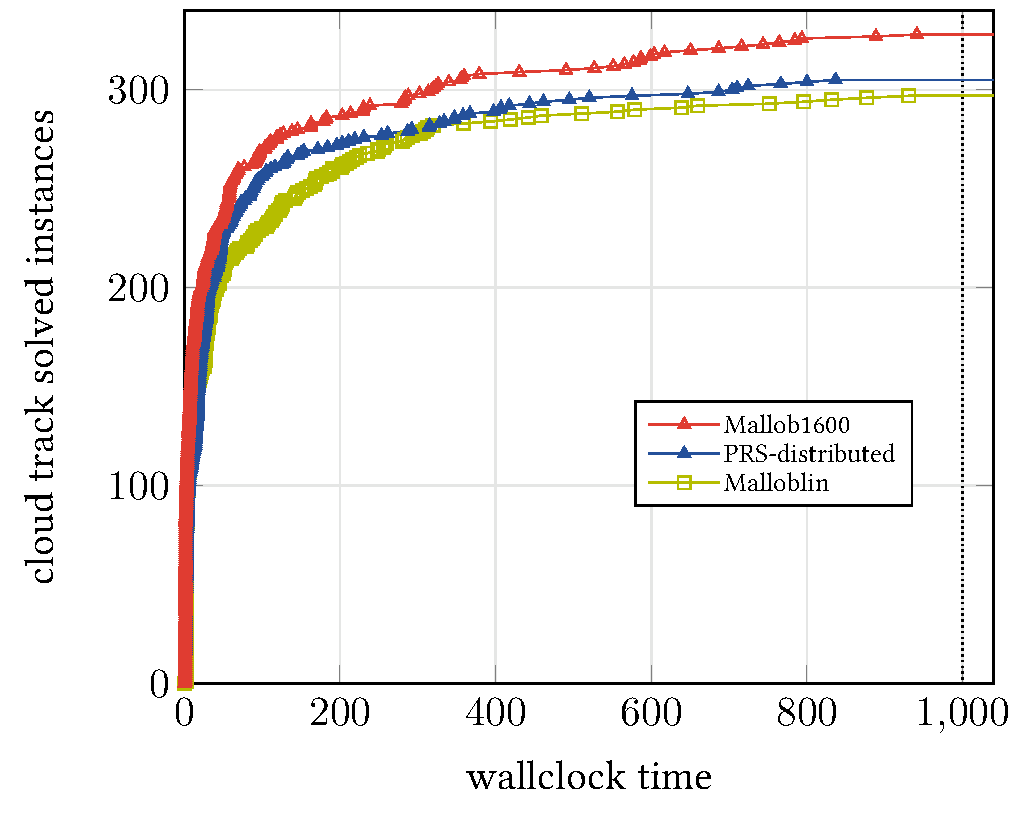
\includegraphics[width=.95\linewidth]{plots/cloud-all-2023.pdf}
\end{frame}

\begin{frame}{Cloud Track SAT Plot}
\centering
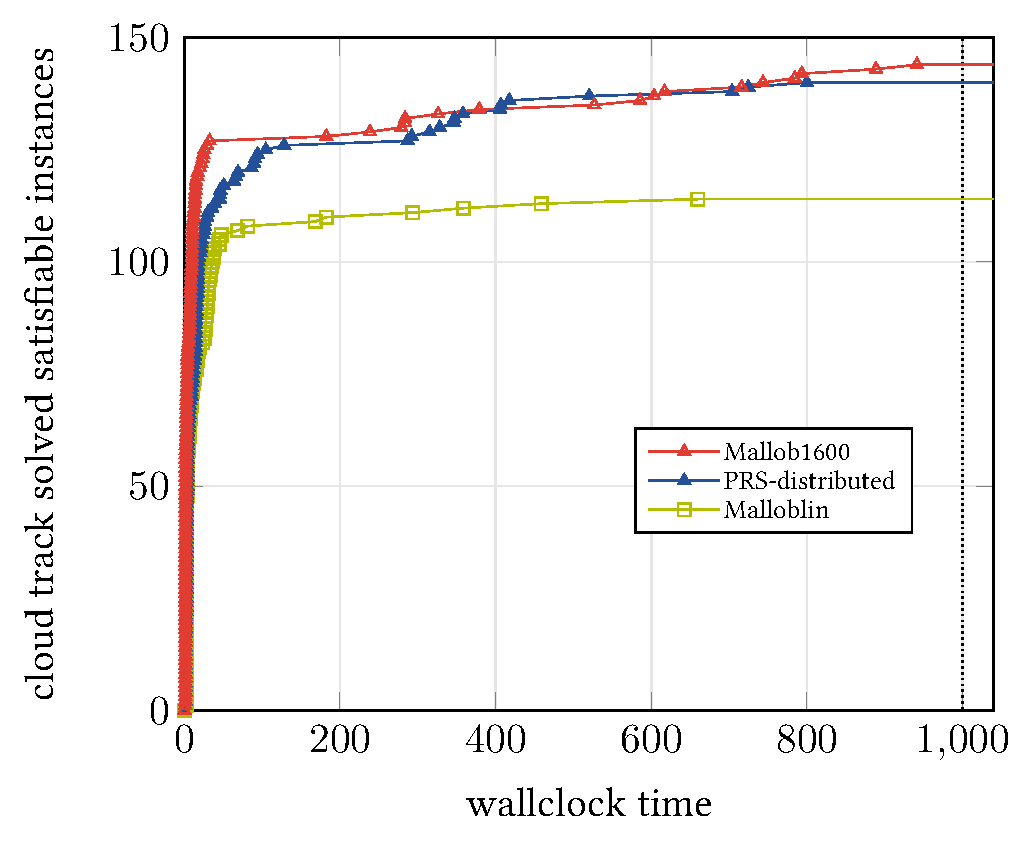
\includegraphics[width=.95\linewidth]{plots/cloud-sat-2023.pdf}
\end{frame}

\begin{frame}{Cloud Track UNSAT Plot}
\centering
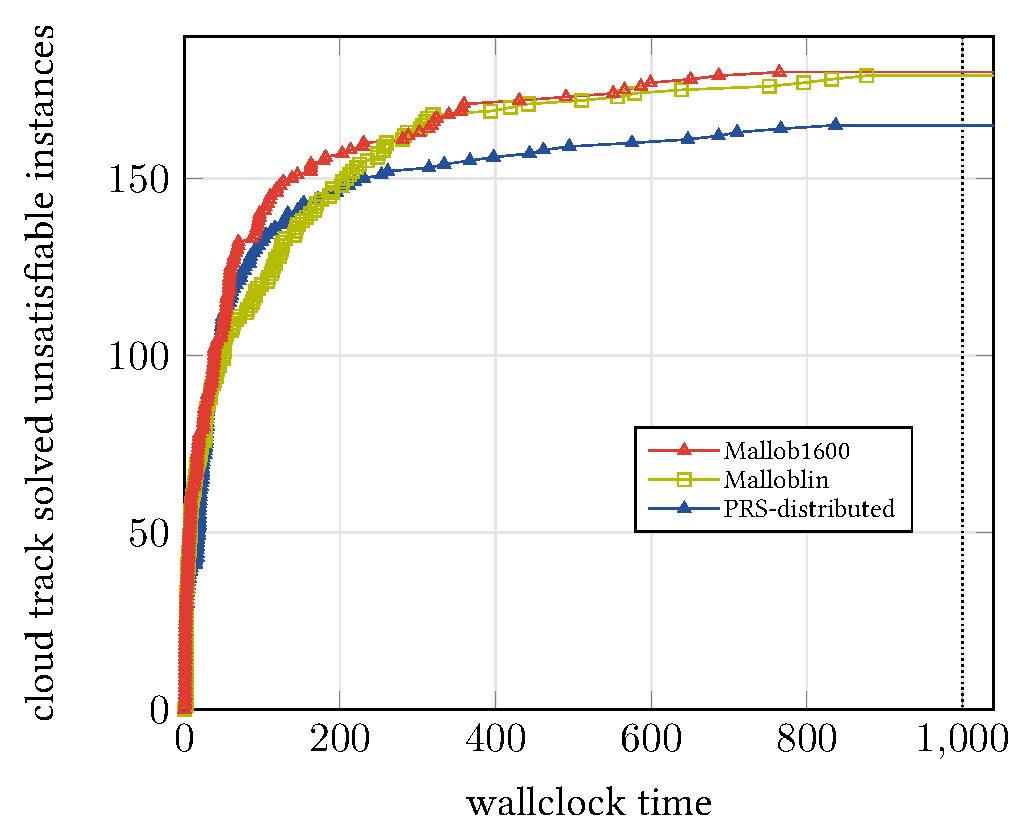
\includegraphics[width=.95\linewidth]{plots/cloud-uns-2023.pdf}
\end{frame}

\begin{frame}{Parallel Track SAT}
%\begin{block}{Winning Solvers}\centering
\renewcommand{\arraystretch}{2}
\begin{tabularx}{\linewidth}{clLrrc}
\toprule
& \bf Solver & \bf Authors & \bf PAR-2 & \bf Solved & \\ \midrule
1 & PRS-parallel & Zhihan Chen, Xindi Zhang, Yuhang Qian and Shaowei Cai & 1143.56 & 143 & \\[1em]
2 & Mallob64 & Dominik Schreiber & 1505.21 & 137 & \\ 
3 & pKisDS-step & Zhihui Xie, Xu Liu, Wanqian Luo, Junhua Huang, Hui-Ling Zhen, Xijun Li, Mingxuan Yuan and Shuai Li & 1796.61 & 132\\
\bottomrule
\end{tabularx}
%\end{block}
\end{frame}

%PRS, 793.97, 143
%Mallob64, 1219.77, 136
%pKisDS-step, 1527.02, 131
%satcomp-nopre-prs,1633.31
%mallob23-parallel-1,1634.1511447368423
%nps-satcomp2023,1689.296532894737
%dps-satcomp2023,1717.342447368421
%satcomp-pkissat,1730.0069934210524
%satcomp-pkissat-str,1740.795375
%satcomp-pkisds,1747.1895986842108
%gimsatul,1976.1754210526315
%satcomp-mergesat,2196.4121513157893
%pahkis23,2318.3461447368422
%pakisinc23,2700.0586907894735
%satcomp-solimul-parallel,3239.0339210526313

\begin{frame}{Parallel Track SAT Plot}
\centering
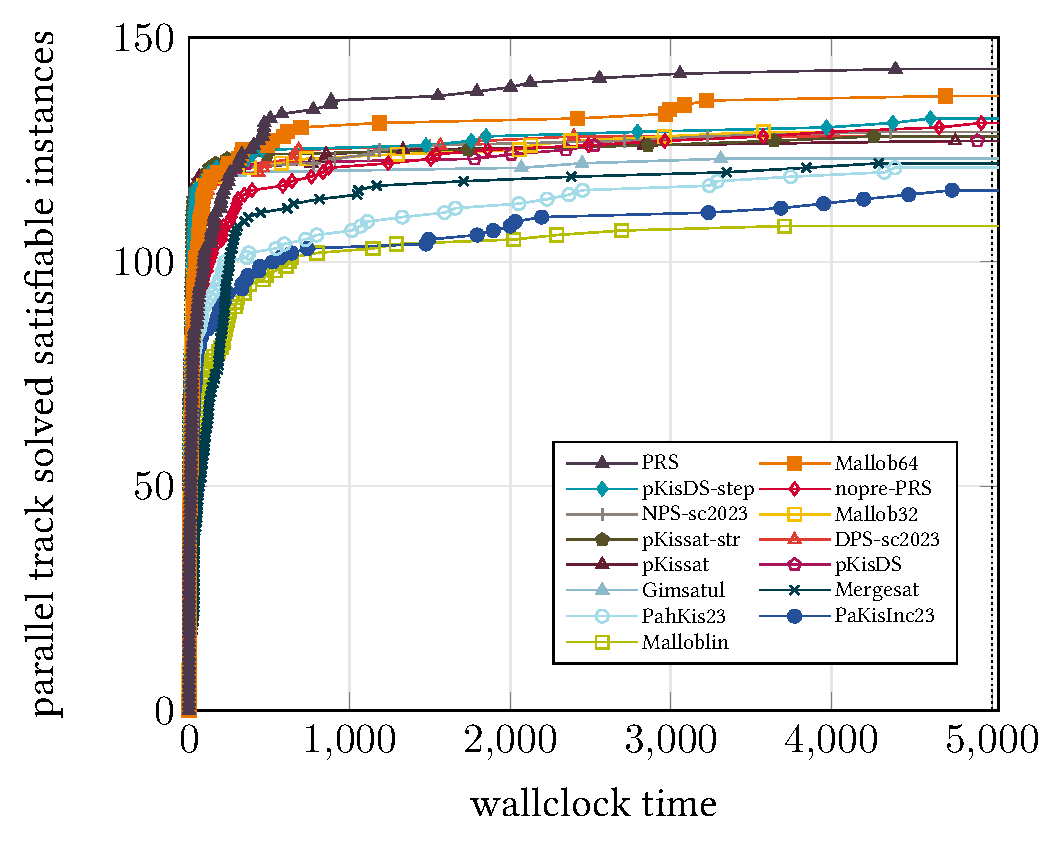
\includegraphics[width=.95\linewidth]{plots/parallel-sat-2023.pdf}
\end{frame}

\begin{frame}{Parallel Track UNSAT}
%\begin{block}{Winning Solvers}\centering
\renewcommand{\arraystretch}{2}
\begin{tabularx}{\linewidth}{clLrrc}
\toprule
& \bf Solver & \bf Authors & \bf PAR-2 & \bf Solved & \\ \midrule
1 & PRS-parallel & Zhihan Chen, Xindi Zhang, Yuhang Qian and Shaowei Cai & 1455.86 & 177 & \\ 
2 & Malloblin & Md Solimul Chowdhury & 1501.29 & 176 & \\ 
3 & p-Kissat & Vincent Vallade, Julien Sopena and Souheib Baarir & 1852.87 & 170 & \\ 
\bottomrule
\end{tabularx}
%\end{block}
\end{frame}

%Malloblin,1204.22, 172
%PRS,1228.23, 172
%pKissat,1562.28, 166
%satcomp-pkissat-str,1615.0146489361703
%satcomp-pkisds-step,1816.3130319148936
%satcomp-pkisds,1904.435659574468
%mallob23-parallel-2,1932.0829202127659
%mallob23-parallel-1,1965.3824308510639
%satcomp-nopre-prs,2036.0646702127663
%gimsatul,2420.2167765957447
%pakisinc23,2517.566069148936
%pahkis23,2551.708340425532
%nps-satcomp2023,2687.345085106383
%dps-satcomp2023,2720.1612021276596
%satcomp-mergesat,4906.67154787234

\begin{frame}{Parallel Track UNSAT Plot}
\centering
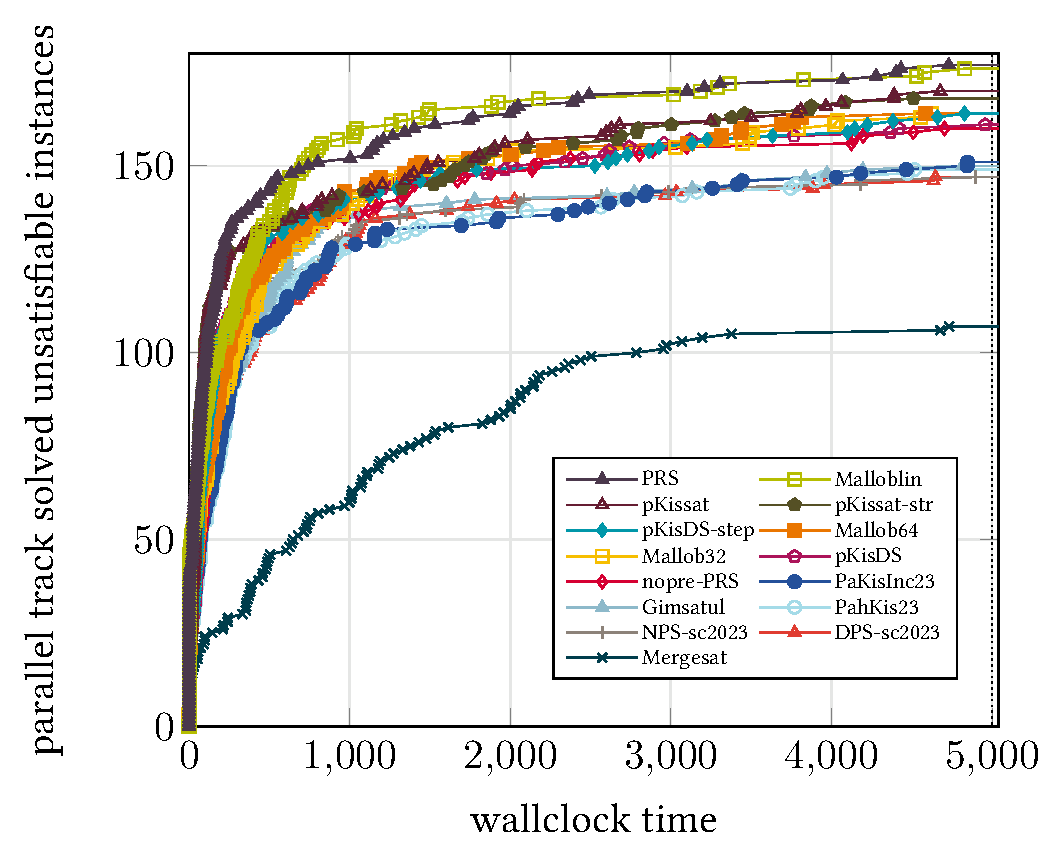
\includegraphics[width=.95\linewidth]{plots/parallel-uns-2023.pdf}
\end{frame}

\begin{frame}{Parallel Track}
%\begin{block}{Winning Solvers}\centering
\renewcommand{\arraystretch}{2}
\begin{tabularx}{\linewidth}{clLrrc}
\toprule
& \bf Solver & \bf Authors & \bf PAR-2 & \bf Solved & \\ \midrule
1 & PRS-parallel & Zhihan Chen, Xindi Zhang, Yuhang Qian and Shaowei Cai & 2272.36 & 320 & \\ 
2 & Mallob64 & Dominik Schreiber & 2746.30 & 301 & \\ 
3 & p-Kissat & Vincent Vallade, Julien Sopena and Souheib Baarir & 2824.57 & 297 & \\
\bottomrule
\end{tabularx}
%\end{block}

\medskip

\begin{itemize}
\item Same number solved by parallel and cloud track winner\\(64 cores and 5000 seconds vs 1600 cores and 1000 seconds)
\end{itemize}

\end{frame}


%PRS,1738.73, 315 
%Mallob64, 2272.73, 295
%pKissat, 2294.50, 293
%satcomp-pkissat-str,2325.8093523035227
%satcomp-pkisds-step,2340.306590785908
%mallob23-parallel-1,2460.387184281843
%satcomp-pkisds,2475.898978319783
%satcomp-nopre-prs,2496.050533875339
%satcomp-solimul-parallel,2733.6742899728997
%gimsatul,2833.0065528455284
%nps-satcomp2023,2850.932111111111
%dps-satcomp2023,2879.204222222222
%pahkis23,3040.9479186991875
%pakisinc23,3180.789544715448
%satcomp-mergesat,4190.53901897019


\begin{frame}{Parallel Track ALL Plot}
\centering
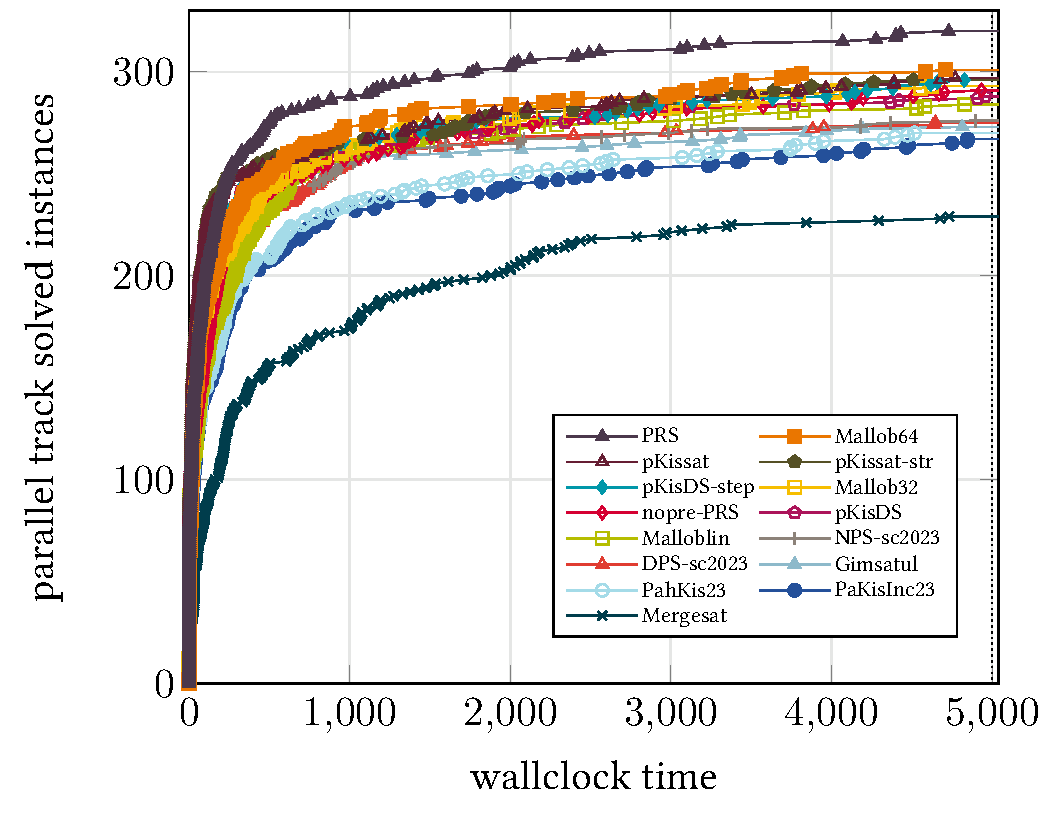
\includegraphics[width=.95\linewidth]{plots/parallel-all-2023.pdf}
\end{frame}



\begin{frame}{Main (Sequential) Track SAT}
%\begin{block}{Winning Solvers}\centering
\renewcommand{\arraystretch}{1.6}
\begin{tabularx}{\linewidth}{clLrrc}
\toprule
& \bf Solver & \bf Authors & \bf PAR-2 & \bf Solved & \\ \midrule
1 & SBVA-CaDiCaL & Andrew Haberlandt and Harrison Green  & 2337.38 & 123 & \\ 
2 & CaDiCaL-Scavel & Zhihui Li, Guanfeng Wu, Yang Xu, Keming Wang, Zhiguo Long and Zhibin Yu & 2351.34 & 122 & \\ 
3 & CaDiCaL-vivinst & Armin Biere, Mathias Fleury and Florian Pollitt & 2359.31 & 122 &\\
\bottomrule
\end{tabularx}
%\end{block}
\end{frame}


%SBVA-CaDiCaL,2337.38
%CaDiCaL_rel_1.5.3.Scavel,2351.34
%CaDiCaL_vivinst,2359.31
%Cadical_ESA,2441.46
%MapleCaDiCaL_LBD-990_275,2462.5355156818187
%AMSAT_,2540.7415762272726
%MapleCaDiCaL_PPD-500_500,2560.204072194805
%ReEncode-kissat-ReEncode-pair-kissat.sh,2578.982324402597
%kissat-3.1.0,2584.8253838311684

\begin{frame}{Main (Sequential) Track SAT Plot}

\parindent -17pt
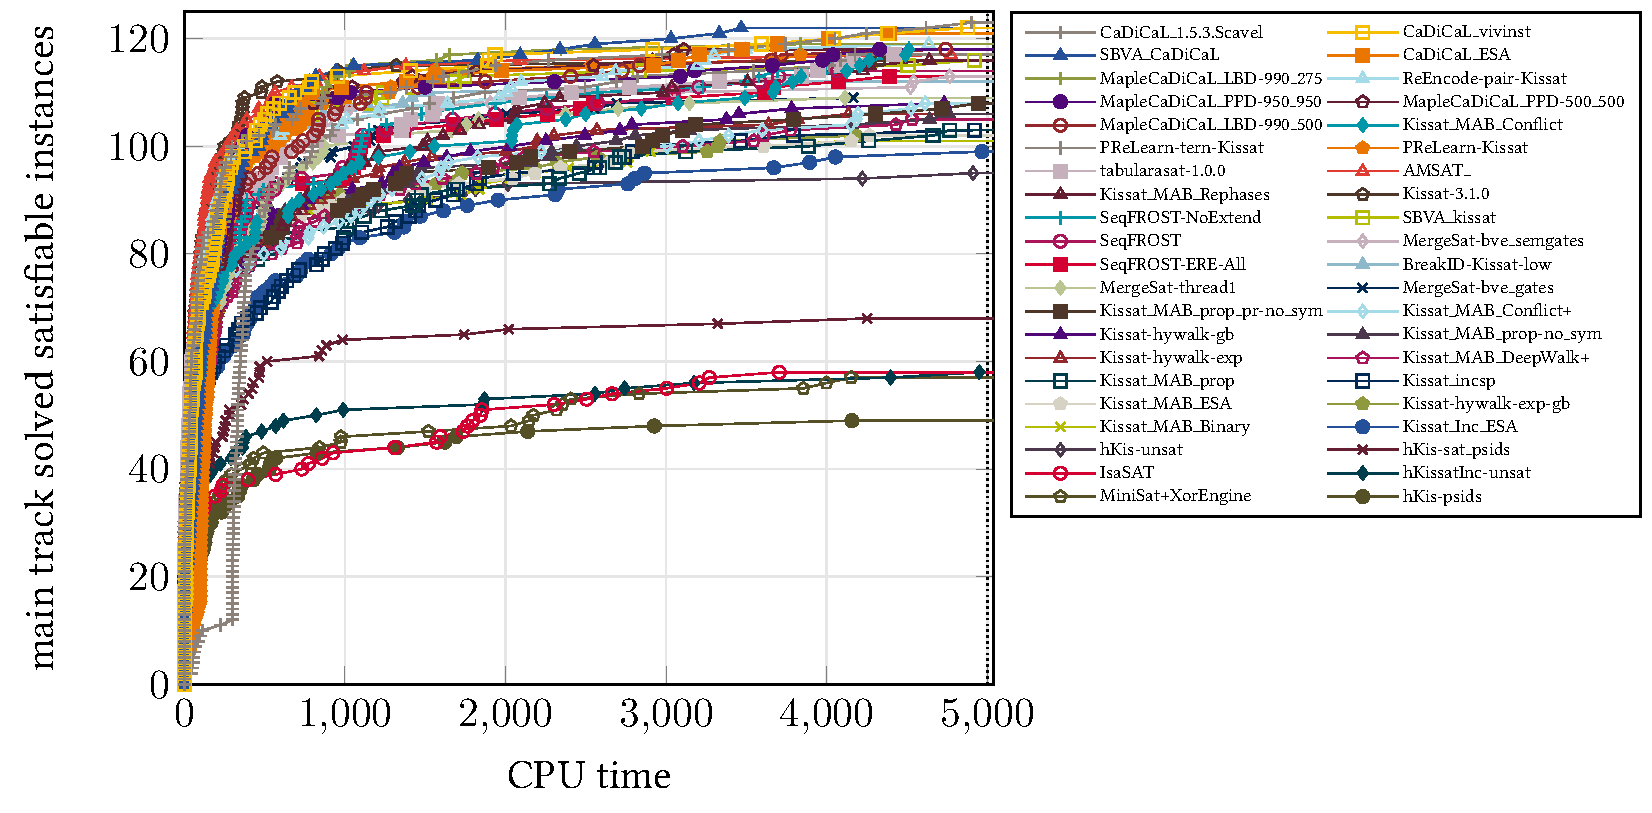
\includegraphics[width=1.1\linewidth]{plots/main-sat-2023.pdf}

\begin{itemize}
\item The Return of CaDiCaL (strongest on satisfiables)
\end{itemize}

\end{frame}

\begin{frame}{Main Sequential Track UNSAT}
%\begin{block}{Winning Solvers}\centering
\renewcommand{\arraystretch}{2}
\begin{tabularx}{\linewidth}{clLrrc}
\toprule
& \bf Solver & \bf Authors & \bf PAR-2 & \bf Solved & \\ \midrule
1 & Kissat-MAB-prop & Yu Gao& 2657.13 & 167 & \\ 
2 & SBVA-CaDiCaL & Andrew Haberlandt and Harrison Green & 2975.11 & 162 & \\ 
3 & PReLearn-Kissat & Joseph Reeves and Randy Bryant & 4016.81 & 142\\
\bottomrule
\end{tabularx}
%\end{block}
\end{frame}


%Kissat_MAB_prop,2657.13,
%Kissat_MAB_prop_pr-no_sym,2831.24,
%Kissat_MAB_prop-no_sym,2892.98,
%SBVA-CaDiCaL,2975.11,
%SBVA-kissat,3852.39,
%PReLearn-Kissat,4016.81,
%MapleCaDiCaL_PPD-500_500,4042.48,
%PReLearn-kissat-PReLearn-tern-kissat.sh,4123.67,

\begin{frame}{Main (Sequential) Track UNSAT Plot}

\parindent -17pt
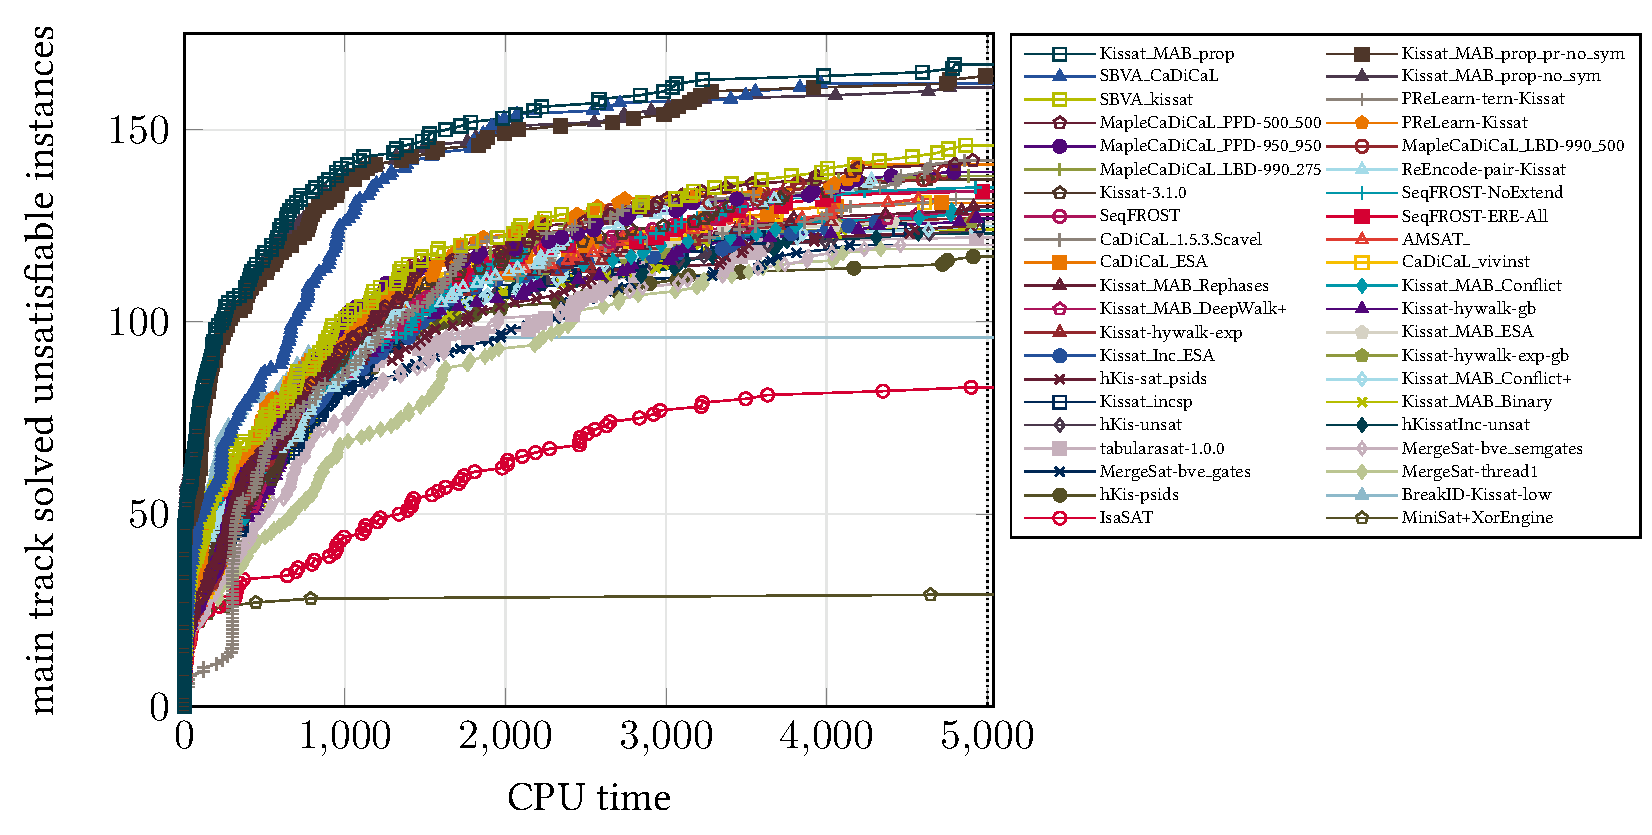
\includegraphics[width=1.1\linewidth]{plots/main-uns-2023.pdf}

\begin{itemize}
\item Beyond Resolution Strikes Back (in all top-tier solvers)
\end{itemize}

\end{frame}


\begin{frame}{Main Sequential Track}
%\begin{block}{Winning Solvers}\centering
\renewcommand{\arraystretch}{1.7}
\begin{tabularx}{\linewidth}{clLrrc}
\toprule
& \bf Solver & \bf Authors & \bf PAR-2 & \bf Solved & \\ \midrule
1 & SBVA-CaDiCaL & Andrew Haberlandt and Harrison Green & 3274.01 & 284 & \\ 
2 & Kissat-MAB-prop* & Yu Gao & 3596.73 & 272 & \\ 
3 & MCaDiCaL-PPD-500 & Jonathan Chung, Sam Buss and Vijay Ganesh & 3933.51 & 260 &\\
\bottomrule  
\end{tabularx}
%\end{block}
\end{frame}

%SBVA-CaDiCaL,3274.01, 284
%Kissat_MAB_prop_pr-no_sym,3596.73, 272
%Kissat_MAB_prop,3614.43, 270
%Kissat_MAB_prop-no_sym,3652.44, 267
%SBVA-Kissat,3882.65, 262
%MapleCaDiCaL_PPD-500_500, 3933.51, 260
%MapleCaDiCaL_LBD-990_275,3952.54
%PReLearn-kissat-PReLearn-kissat.sh,3959.37
%MapleCaDiCaL_PPD-950_950,3997.86
%MapleCaDiCaL_LBD-990_500,4001.53

\begin{frame}{Main (Sequential) Track ALL Plot}

\parindent -17pt
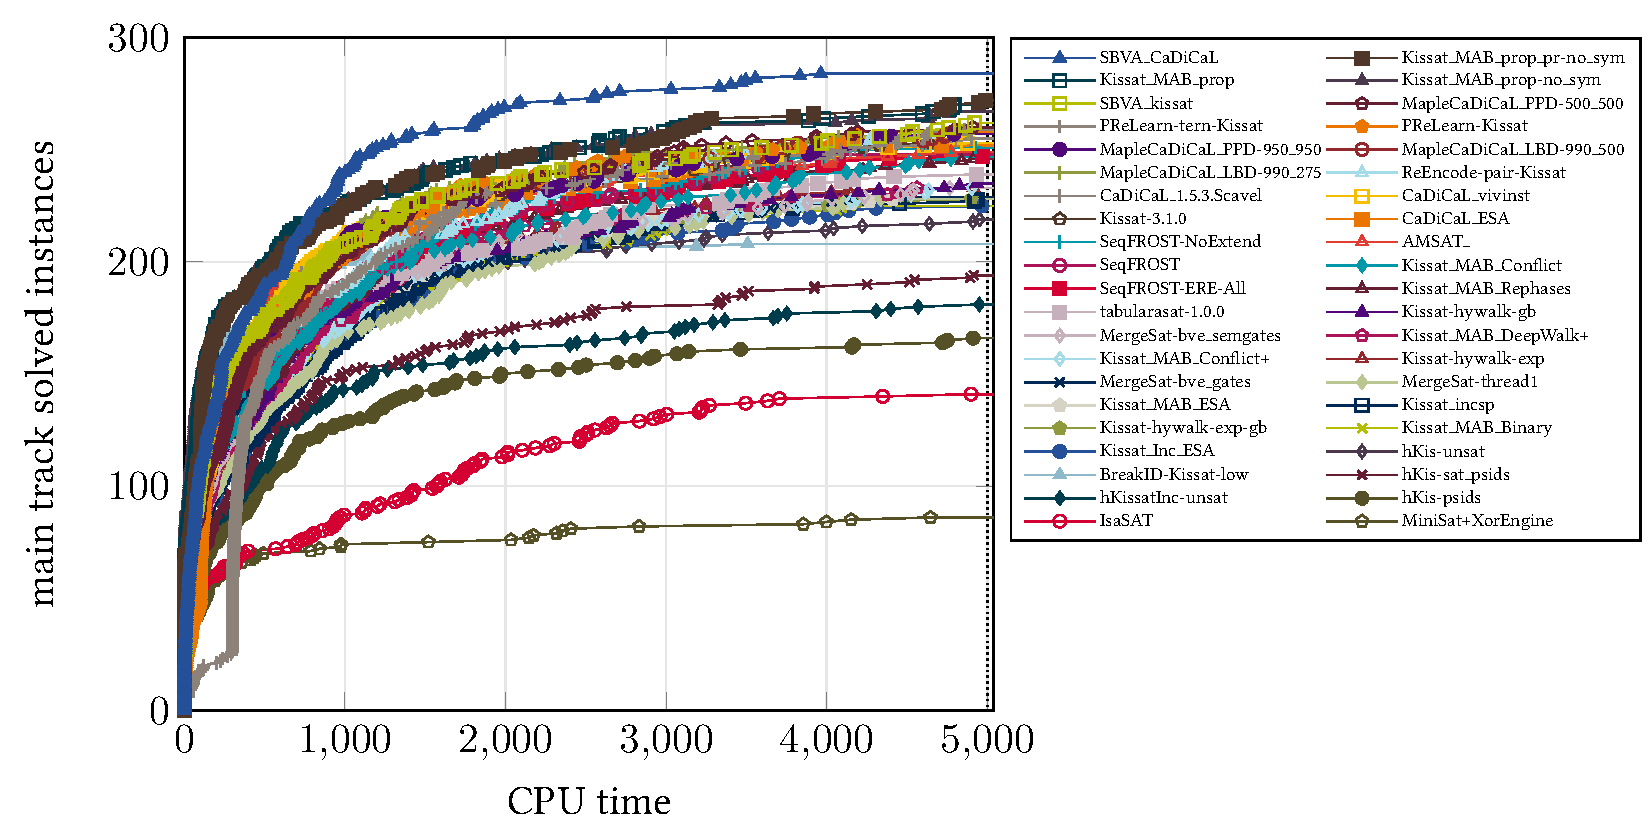
\includegraphics[width=1.1\linewidth]{plots/main-all-2023.pdf}

\begin{itemize}
\item Winner not impacted by own benchmarks
\end{itemize}

\end{frame}


%\begin{frame}{Main Track Winners: Sequential, Parallel, Cloud}
%\centering
%\includegraphics[width=.8\linewidth]{plots/cloud-par-seq-main-2022.pdf}
%\end{frame}


\begin{frame}{CaDiCaL Hack Track}

Winner: \\
CaDiCaL-vivinst by Armin Biere, Mathias Fleury and Florian Pollitt


\end{frame}

\begin{frame}{Special Prize}

What is the ranking if checker timeouts were counted as solved?

\bigskip

~~~~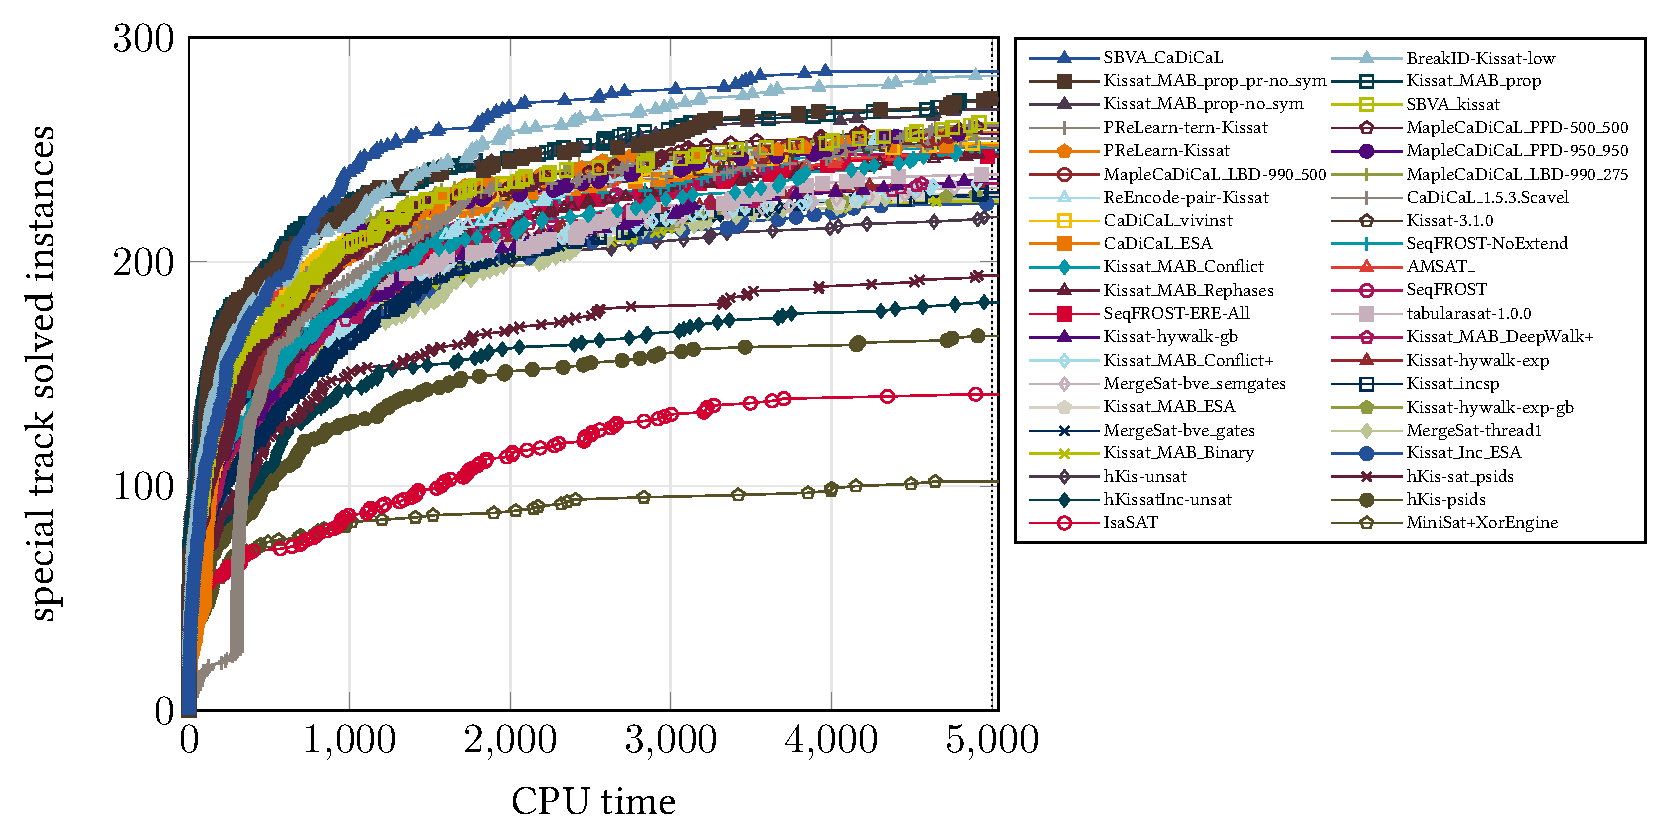
\includegraphics[width=\linewidth]{plots/special-all-2023.pdf}

Special prize: BreakID-kissat by Bart Bogaerts, Jakob Nordström, Andy Oertel and Çağrı Uluç Yıldırımoğlu

\end{frame}

\begin{frame}{Certificate Issues in 2023}
\centering

\begin{itemize}\setlength\itemsep{1em}
	\item Rules do not cover corner cases, esp. for UNSAT certificates
	\begin{itemize}
		\item Proof checker failure (wrong proof/checker issue)
		\item Proof checker timeouts (45k seconds)
	\end{itemize}
	\item New checkers not mature yet
	\item \emph{This will change for 2024}\\[1em]
\begin{tabular}{@{}cc|ccc}
\toprule
Result & Certificate & SAT & UNSAT (2023) & UNSAT (2024) \\ \midrule
Wrong & Wrong & Disq. & Disq. & Disq. \\
Correct & Timeout & Disq. & Unsolved & Unsolved \\
Correct & Wrong & Disq. & Unsolved & \bf Disq. \\
\bottomrule
\end{tabular}
\end{itemize}
\end{frame}

%\begin{frame}{UNSAT Certificates for Parallel Solvers}
%\begin{block}{UNSAT proof certificates will be enforced "sooner than you think"}
%	\begin{itemize}\setlength\itemsep{1em}
%		\item 2022: notable correctness issues with parallel solvers
%		\item \emph{2023 will see a new track (per discussions at PoS 2022)}\\[.5em]
%		\begin{itemize}\setlength\itemsep{1em}
%			\item Incentives for developing proof certification for parallel SAT solvers
%			\item (Perhaps not in 2023 though\dots but soon enough!)
%		\end{itemize}
%	\end{itemize}
%%\end{block}
%\end{frame}

%\begin{frame}{New for 2023: Open Call for Proof Checkers}
%\begin{block}{Support More Powerful Proof Systems}
%\begin{itemize}\setlength\itemsep{.5em}
%\item Call to be released by early September
%\item Intent to submit (incl. extended abstract): early fall
%\item Submission deadline: November 30, 2022 (preliminary)
%\item Checkers announced by January 15, 2023 (preliminary)
%\item \textbf{Requirement:} Checkers must be \emph{formally verified}
%\item Main track UNSAT
%\item \textbf{Implications:}
%\begin{itemize}
%\item Each solver must specify checker  be used to check its proofs
%\item Per-instance time limit on proof checking 
%\item "Solving" an instance requires that  proof can be checked 
%\end{itemize}
%\end{itemize}
%%\end{block}
%\end{frame}
%
%\begin{frame}{New for 2023: Challenge Track (preliminarily planned)}
%\begin{block}{Large Anniversary Track Dataset}
%\begin{itemize}\setlength\itemsep{1em}
%\item Benchmark set public 
%\item Benchmarks: unsolved instances from the 2022 Anniversary track
%\item \textbf{Challenge:} Devise a SAT solver which can solve as many of the benchmark instances
%\begin{itemize}\setlength\itemsep{1em}
%\item "Solved": solved sequentially on StarExec within the 2022 Anniversary track time limit
%\item Results checked by organizers
%\item "Hall of fame": list for each instance authors who solved it and when was the certificate submitted
%\end{itemize}
%\end{itemize}
%%\end{block}
%\end{frame}


\begin{frame}{Thank you!}
\begin{center}
\begin{tikzpicture}[fill=normalbg]
\node[xshift=-2em] (aws) at (current page.north west) { 
\includegraphics[width=12em]{img/AWSlogo.png} };
\node[xshift=-18em] (cas) at (current page.north east) { 
\includegraphics[width=10em]{img/filuta-and-symbol-stacked.png} };
\node[fill=black, xshift=5em, yshift=15em] (sex) at (current page.south west) { 
\includegraphics[width=20em]{img/SEXlogo.png} };
\end{tikzpicture}
\end{center}
\end{frame}


%----------------------------------------------------------------------------------------

\end{document}